% \documentclass[a4paper,11pt]{article}
% \usepackage[hyperref]{beamerarticle}

\documentclass[final]{beamer}

\usepackage[hangul]{kotex}
\usepackage{amsfonts,amsmath,xob-amssymb}

\usepackage{amsthm}
\newtheorem{defn}{Definition}
\newtheorem{thm}{Theorem}

\usepackage{cancel}
\graphicspath{{./_img/02/}}

\usepackage{graphicx}
\usepackage{media9}

\mode<presentation>{
	\usetheme{Madrid}
	\usecolortheme{default}
	\usefonttheme{professionalfonts}
}

\def\b{\boldsymbol}

\mode<article>{
\usepackage{fullpage}
}
\usepackage{ulem}

\newcommand{\bb}{\mathbb}
\newcommand{\bd}{\mathbf}
\newcommand{\p}{\partial}

\newcounter{saveenumi}
\newcommand{\seti}{\setcounter{saveenumi}{\value{enumi}}}
\newcommand{\conti}{\setcounter{enumi}{\value{saveenumi}}}

\newcommand{\mail}{\url{mailto:experiment.namun+2016f@gmail.com} }


\title{게임이란 무엇인가?}
\subtitle{우리 곁의 게임들}
\author[조남운]{허준석$\rightarrow$이동한$\rightarrow$\emph{조남운}\\\mail}

\begin{document}

\begin{frame}[t]{}
	\titlepage
\end{frame}
%--- Next Frame ---%

\begin{frame}[t]{목차}
	\tableofcontents
\end{frame}
%--- Next Frame ---%

\section{우리 곁의 게임들} % (fold)
\label{sec:GamesInPractice}

\begin{frame}[t]{2012 대통령 선거}
	\begin{itemize}
		\item 두 후보 사이의 단일화 과정  
		\item 이 과정에는 어떤 게임들이 개입되어 있었을까?
	\end{itemize}
\end{frame}
%--- Next Frame ---%

\begin{frame}[t]{치킨 게임}
	\begin{center}
		\framebox{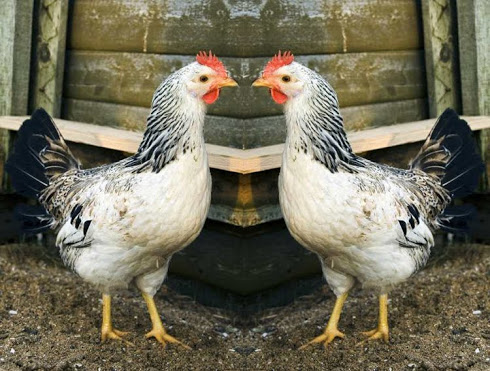
\includegraphics[width=0.5\linewidth]{image_01.png}}
	\end{center}
	$\checkmark$ \href{http://www.youtube.com/watch?v=u7hZ9jKrwvo}{Rebel Without a Cause} \\
	$\checkmark$ \href{http://www.youtube.com/watch?v=6L-IbkWHsOE}{Stand by Me}
\end{frame}
%--- Next Frame ---%

\begin{frame}[t]{다리에 불을 질러라!}
	\begin{columns}[c]
		\column{0.45\linewidth}
		\framebox{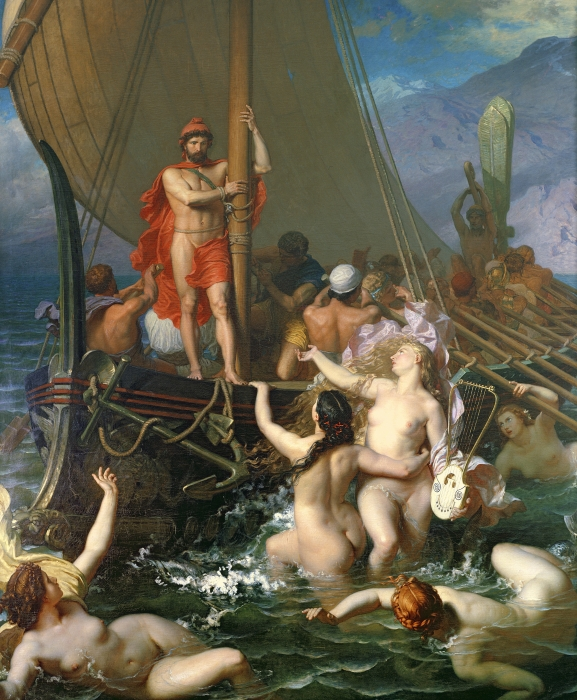
\includegraphics[width=0.9\linewidth]{image_02.png}}
		\column{0.45\linewidth}
		\begin{itemize}
			\item 문 후보는 협상에 앞서 민주당의 후보가 되었고, 안 후보 역시 출마를 선언
			\item 왜 불을 지르는 것이 유리할까?
			\item 때로는 선택의 여지는 없애는 편이 더 낫다. 
			\item 적군-아군 \\ 그리고 지도자-추종자
		\end{itemize}
	\end{columns}
\end{frame}
%--- Next Frame ---%

\begin{frame}[t]{Dr. Strangelove}
	\begin{columns}[c]
		\column{0.45\linewidth}
		\framebox{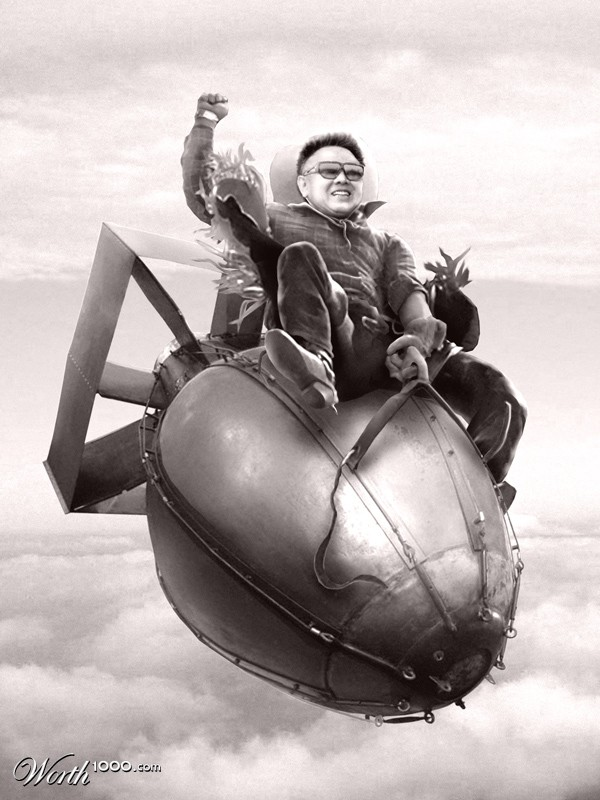
\includegraphics[width=0.9\linewidth]{kim.jpg}}
		\column{0.45\linewidth}
		\begin{itemize}
			\item "둠스데이머신"이란 무엇인가? 
			\item "rational to be irrational."
			\item 북한의 전략을 이런 면에서 돌아본다면?
		\end{itemize}
	\end{columns}
\end{frame}
%--- Next Frame ---%

\begin{frame}[t]{최후통첩게임 실습}
	\begin{itemize}
		\item \url{} // heroku
		\begin{itemize}
			\item name: 본인의 이름
			\item pw: 본인의 학번
		\end{itemize}
		\item 임의의 두 사람과 매칭될 것임. 
		\item 제안하는 사람: 
		\begin{itemize}
			\item 1000 ECU (Experimental Currency Unit) 을 분배
		\end{itemize}
		\item 제안받는 사람:
		\begin{itemize}
			\item 위 제안을 수락: 제안한 금액을 둘이 나눠가짐
			\item 위 제안을 거절: 양쪽 모두 0 ECU
		\end{itemize}
		\item 동일 게임을 파트너를 바꿔 다시 시행 (결국 서로 다른 상대와 제안측, 제안받는 측을 한번씩 수행하게 됨)
	\end{itemize}
\end{frame}
%--- Next Frame ---%

\begin{frame}[t]{최후통첩게임 (Ultimatum Game)}
	\begin{columns}[c]
		\column{0.45\linewidth}
		\framebox{
\includegraphics[width=0.9\linewidth]{image_03.png}}
		\column{0.45\linewidth}
		\begin{itemize}
			\item 먼저 제안하는 쪽이 유리할까?
			\item 실제로 이 상황에 있다면 당신의 선택은?
			\item 이성과 감정 
		\end{itemize}
	\end{columns}
\end{frame}
%--- Next Frame ---%

\begin{frame}[t]{누구나 매일 하는 최후 통첩 게임}
	\begin{itemize}
		\item 판매자: 제안자 - A 라는 상품을 $p$ 만큼의 화폐와 교환할 것을 제안
		\item 구매자: 수용자 - 위 제안을 받아들이기 / 거절하기
		\item 거절할 경우 양쪽의 payoff는 모두 0 
		\item 수용할 경우
		\begin{itemize}
			\item 판매자: A상품의 판매 이윤 ($p$ - A 비용)
			\item 구매자: A상품의 구매 이득 (A에 대해 느끼는 구매자의 가치 - $p$)
		\end{itemize}
	\end{itemize}
\end{frame}
%--- Next Frame ---%

\begin{frame}[t]{대선 2012: 경쟁 결과}
	\begin{columns}[c] % contents are top vertically aligned
		\begin{column}[T]{5cm} % each column can also be its own environment
		\begin{itemize}
			\item 초협력자? 자기희생?
			\item 이후를 생각한 고도의 전략? \\ (결국 질게 없는 싸움?)
		\end{itemize}
		\end{column}
		\begin{column}[T]{5cm} % alternative top-align that's better for graphics
			\framebox{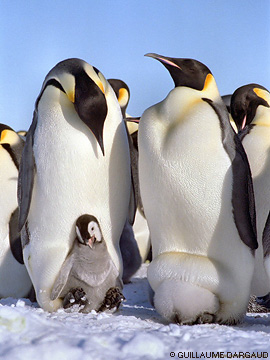
\includegraphics[width=0.9\linewidth]{image_04.png}}
		\end{column}
	\end{columns}
\end{frame}
%--- Next Frame ---%

\begin{frame}[t]{Golden Balls}
	\begin{enumerate}
		\item 100개의 골든볼 (10파운드-7만 5천 파운드) 중 12개가 꼽히고 4개의 "킬러볼" 포함. 16개를 네명의 참가자에게 임의로 배분. 각자 두 개를 앞 쪽(모두 볼 수 있음)에 두 개를 뒤에 둠. 
		\item 뒤에 둔 공에 적힌 액수를 말하는데, 거짓말 가능. 누가 거짓말을 말하고 있는지 토의한 후 한 명을 지목 (동률일 때는 해당 자만 놓고 다시 토의하거나 아니면 무작위로 결정)하여 탈락. 각자 공의 액수를 공개하고 제외된 참가자의 공은 영원히 게임에서 제외됨. 
		\seti
	\end{enumerate}
\end{frame}
%--- Next Frame ---%

\begin{frame}[t]{Golden Balls}
	\begin{enumerate}
	 \conti
	 \item 두번째 라운드에서 세 명의 참가자들의 공은 다시 기계로 돌아간다. 이제 14개의 공을 뽑고 1개의 킬러볼을 넣어 15개를 만든 후 이를 세 명의 참가자에게 배분. 두 개는 앞 쪽에 세 개는 뒷쪽에 놓고 앞의 과정을 반복한다. 
	\item 두 명이 남았을 때 10개의 공을 뽑고 1개의 킬러볼을 넣고 11개의 공을 두고 마주 앉는다. 둘이서 버릴 공과 잭팟으로 적립할 공을 차례로 뽑아나간다. 이때 적립할 공으로 킬러볼이 선택되면 그간 쌓인 잭팟의 가치는 1/10이 된다. 이렇게 5개까지 뽑아 나간다. 
	\conti
	\end{enumerate}
\end{frame}
%--- Next Frame ---%

\begin{frame}[t]{Golden Balls}
	\begin{enumerate}
		 \conti
		 \item 이렇게 공을 다 뽑은 후 둘은 "split"과 "steal" 중 하나를 동시에 선택한다. 만일 둘 다 "split"을 택하면 잭팟은 1/2로 나뉘 가진다. 둘다 steal을 택하면 0, 한 명은 steal, 다른 한 명은 split이면 steal을 한 사람이 100{\%}를 가져간다.  
		\seti
	\end{enumerate}
	\vspace{5mm}
	\begin{center}
		\framebox{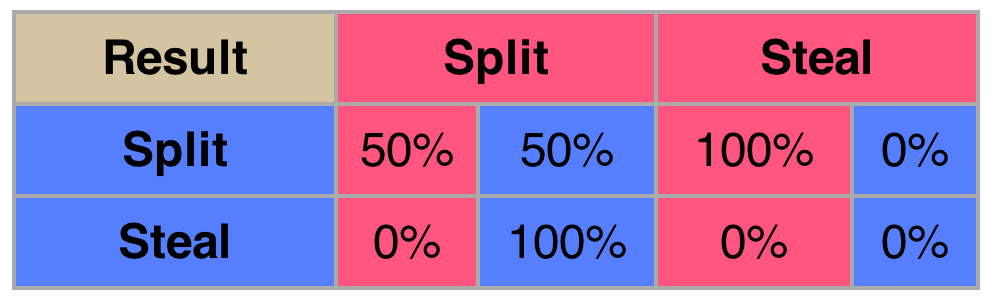
\includegraphics[width=0.6\linewidth]{image_05.png}}
	\end{center}
\end{frame}
%--- Next Frame ---%

\begin{frame}[t]{실제 사례}
	\begin{columns}[t] % contents are top vertically aligned
		\begin{column}{0.5\linewidth} % each column can also be its own environment
		\begin{itemize}
			\item \href{http://www.youtube.com/watch?v=p3Uos2fzIJ0}{협상에 매력을 활용하기}
			\item \href{http://www.youtube.com/watch?v=S0qjK3TWZE8}{또라이 전략}
		\end{itemize}
		\end{column}
		\begin{column}[T]{0.5\linewidth} % alternative top-align that's better for graphics
			\framebox{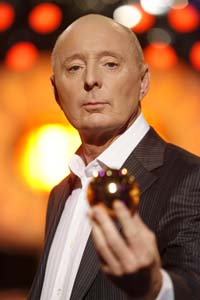
\includegraphics[width=0.6\linewidth]{image_06.png}}
		\end{column}
	\end{columns}
\end{frame}
%--- Next Frame ---%

% \begin{frame}[t]{우리도 해보자.}
% 	\begin{itemize}
% 		\item
% 	\end{itemize}
% \end{frame}
%--- Next Frame ---%

\begin{frame}[t]{페널티킥}
	\begin{center}
		\framebox{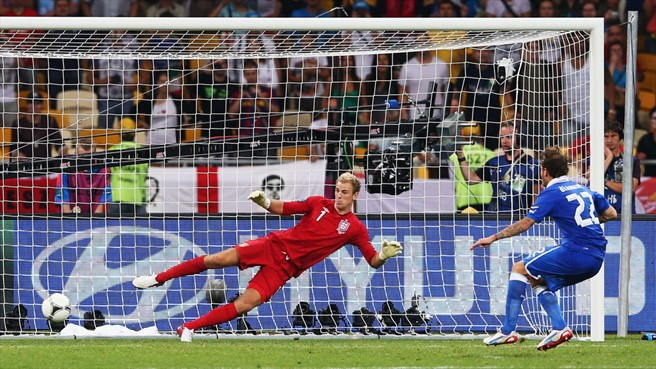
\includegraphics[height=0.3\textheight]{image_07.png}}
	\end{center}
	\begin{itemize}
		\item 페널티 킥은 심리전? 
		\item 고도의 게임적 상황! 
		\item 오른쪽, 가운데, 왼쪽 / 상,중,하 
	\end{itemize}
\end{frame}
%--- Next Frame ---%

% section GamesInPractice (end)

\section{게임이론이란 무엇인가?} % (fold)
\label{sec:WhatisGame}

\begin{frame}[t]{게임은 혼자하지 않는다}
	\begin{center}
		\framebox{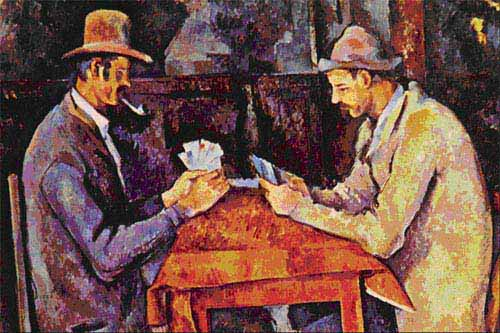
\includegraphics[width=0.6\linewidth]{image_08.png}}
	\end{center}
	\begin{itemize}
		\item 게임은 혼자하지 않는다. 
		\item 그 결과는 내가 한 것만으로 결정되지 않는다. 
	\end{itemize}
\end{frame}
%--- Next Frame ---%

\begin{frame}[t]{누가 이기고 누가 지는가?}
	\begin{itemize}
		\item 여러가지 선택지와 전략이 주어지면, 우리는 이기기 위해 최선을 다한다.  
		\item 세상에는 이기는 패턴이 있을까? 
		\item 여러분의 이기는 패턴은? 
		\item 이기는 패턴에 대한 연구가 바로 ``게임이론''!
	\end{itemize}
\end{frame}
%--- Next Frame ---%

% section WhatisGame (end)

\end{document}